% In a path-connected space, a path alpha between basepoints x_1, x_2 conjugates
% loops. Source: book/tex/topology/fundamental-group.tex (§ Fundamental groups).
\documentclass[border=2mm]{standalone}
\usepackage{tikz}
\usetikzlibrary{arrows.meta}
\begin{document}
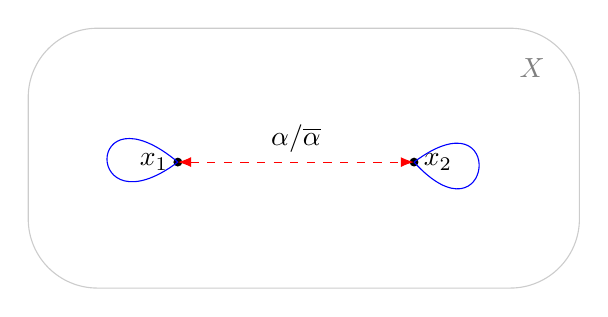
\begin{tikzpicture}[scale=1]
  \draw[rounded corners=25pt, gray!40] (-3.4,-1.6) rectangle (3.6,1.7);
  \node[gray] at (3,1.2) {$X$};
  \fill (-1.5,0) circle (1.6pt) node[left] {$x_1$};
  \fill (1.5,0) circle (1.6pt) node[right] {$x_2$};
  \draw[blue] (-1.5,0) .. controls (-2.7,-0.9) and (-2.7,1) .. (-1.5,0);
  \draw[blue] (1.5,0) .. controls (2.5,-1.1) and (2.7,0.9) .. (1.5,0);
  \draw[red,dashed,{Latex}-{Latex}] (-1.5,0) -- (1.5,0);
  \node[above] at (0,0) {$\alpha/\overline{\alpha}$};
\end{tikzpicture}
\end{document}
